\documentclass[DM,authoryear,toc]{lsstdoc}
% lsstdoc documentation: https://lsst-texmf.lsst.io/lsstdoc.html
\input{meta}

% Package imports go here.

% Local commands go here.

%If you want glossaries
%\input{aglossary.tex}
%\makeglossaries

\title{Calibration Generation, Verification, Acceptance, and Certification.}

% Optional subtitle
% \setDocSubtitle{A subtitle}

\author{%
Chris Waters
}

\setDocRef{DMTN-222}
\setDocUpstreamLocation{\url{https://github.com/lsst-dm/dmtn-222}}

\date{\vcsDate}

% Optional: name of the document's curator
% \setDocCurator{The Curator of this Document}

\setDocAbstract{%
This technote defines the best practices to be used for calibration generation, the verification that that calibration meets requirements, and when deciding if the calibration should be accepted for use in processing at both the summit and USDF.
}

% Change history defined here.
% Order: oldest first.
% Fields: VERSION, DATE, DESCRIPTION, OWNER NAME.
% See LPM-51 for version number policy.
\setDocChangeRecord{%
  \addtohist{1}{2022-03-21}{Initial draft.}{Chris Waters}
  \addtohist{2}{2022-09-16}{Corrected and clarified draft.}{Chris Waters}
  \addtohist{3}{2024-04-17}{Updated draft reflecting processes actually in use.}{Chris Waters}
}


\begin{document}

% Create the title page.
\maketitle
% Frequently for a technote we do not want a title page  uncomment this to remove the title page and changelog.
% use \mkshorttitle to remove the extra pages

% ADD CONTENT HERE
% You can also use the \input command to include several content files.

\section{Introduction}

The purpose of this technote is to provide guidance on the procedures that are used for the construction and management of calibrations.  These guidelines shall be followed for any calibration that will be added to the main butler repositories.  For the purposes of this document, we will consider three cases of calibrations.

\begin{itemize}
\item Calibrations generated for widespread use, using the main butler repository.  These will be called ``combined calibrations'' below, and indicate those calibrations that are used for science processing.
\item Curated calibrations that are defined by an \verb|obs_| package and must be ingested to the butler repository, as they cannot be generated from raw data.  The camera geometry calibration is an example of this type of calibration.
\item Calibrations that have been exported from one butler repository for use in another.
\end{itemize}

Additional private calibrations produced for tests may also exist, but as those will only exist in a user-space collections, they will not be discussed further in this document.

Briefly, calibration construction involves the following steps:
\begin{description}
\item[Generation] An appropriate set of exposures is chosen and processed through the correct \verb|cp_pipe| pipeline.
\item[Verification] The proposed calibration is used to process exposures through the matching \verb|cp_verify| pipeline.  The exposures for generation should be included (the ``in-group'' exposures) to check for problem inputs that indicate the calibration should be remade without those problems, and a set of additional ``out-group'' exposures to check the time stability of the calibration.  This pipeline will soon produce a verification report that will be supplied to the Telescope And auXiliary Instrumentation Calibration Acceptance Board (TAXICAB).
\item[Certification] The proposed calibration is certified for a particular usage date range.  These are generally open ended, with only the start date defined.
\item[Approval] The TAXICAB considers the proposed calibration or calibrations and their associated verification results, and makes the decision on whether the proposal is accepted for use.
\item[Distribution] The collection containing the new calibrations are included in the main calibration collection chain, for all repositories that need the updated calibration.
\end{description}

Figure \ref{fig:flowchart} displays the relationship between the various stages of construction, validation, and use of combined calibrations.

\begin{figure}
  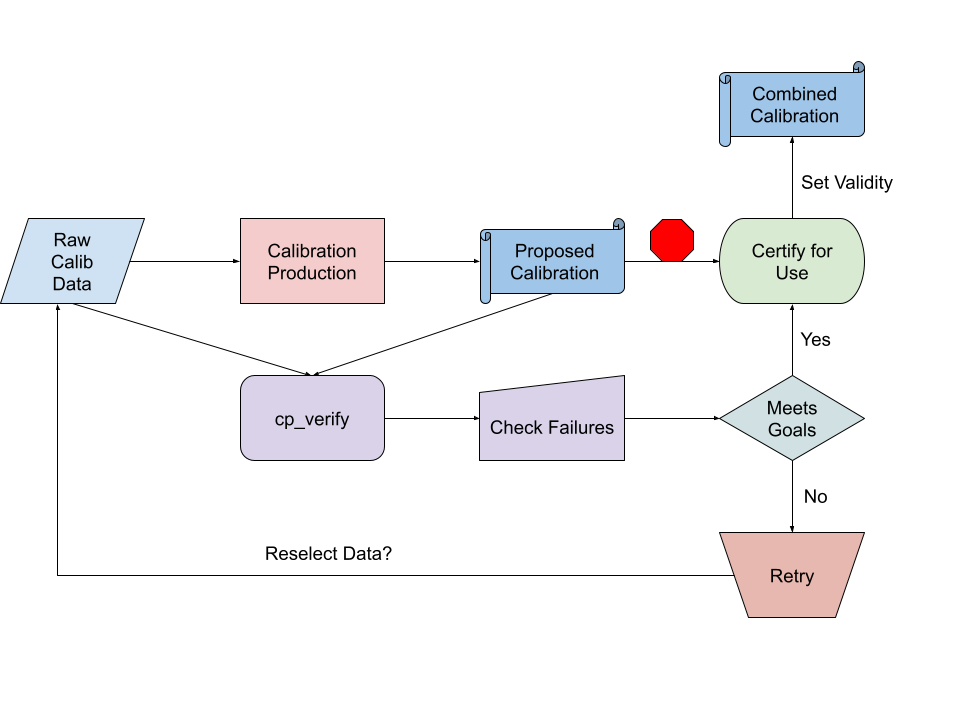
\includegraphics[width=\linewidth]{figures/flowchart.png}
  \caption{Flowchart of the calibration construction process.}
  \label{fig:flowchart}
\end{figure}

\subsection{Collection naming}

Consistent collection names will make the management of calibrations easier.  JIRA tickets will be used to ensure that these collection names are unique, and that there is a location to find the construction artifacts for later analysis.  In addition to this ticket, a short string explaining the purpose of the calibration set should be included in the collection name to provide a human readable ``tag.''  The following collection name patterns, based on the recommendations in \citedsp{DMTN-167} should be followed for all calibrations that will be approved by the TAXICAB.

The calibration generation should use the form
\begin{verbatim}
  $INSTRUMENT/calib/$TICKET/$TAG/${CALIB_TYPE}Gen.${RERUN_ITERATION}
\end{verbatim}
where \verb|$INSTRUMENT| is the camera name, \verb|$TICKET| is the JIRA ticket value, \verb|$TAG| is the short human readable string, \verb|$CALIB_TYPE| is the calibration type being generated, and \verb|$RERUN_ITERATION| is a date string of the form \verb|YYYYMMDDv| indicating when the calibration was made, with a trailing character to be incremented if the generation must be retried.  As an example, a hypothetical new bias would have a collection name like \verb|LATISS/calib/DM-12345/voltageChange/biasGen.20220915a|.

For verification, a similar form is used
\begin{verbatim}
  $INSTRUMENT/calib/$TICKET/$TAG/verify${CALIB_TYPE}.$RERUN_ITERATION}
\end{verbatim}
with the same elements as for generation.


\section{New Combined Calibrations Construction}

A record of the calibration construction process should be retained and attached to the JIRA ticket managing the work, with all commands executed and exposure selections recorded.  Having this record will allow for understanding what happened during construction, in case the final products have problems.

\subsection{Generation}

Combined calibrations will be generated directly from raw exposures as much as possible.  The tasks and pipelines in the \verb|cp_pipe| package can produce all of the calibrations that are currently used for image processing, and can be supplemented as new corrections are developed.  The main documentation for calibration construction is included in \verb|cp_pipe| at \url{https://pipelines.lsst.io/v/daily/modules/lsst.cp.pipe/constructing-calibrations.html}, but the main points will be summarized here.

Calibrations are inter-dependent, and so the construction of one type may require precursor calibrations to be built first.  Figure \ref{fig:dependence} shows the current dependence, with each box pointing to the calibrations that they depend on.  The result of this is that changes in one calibration (such as the gains derived from the photon transfer curve) require other calibrations (the linearity, the brighter-fatter kernel, and the charge transfer inefficiency) to be built as well.

\begin{figure}
  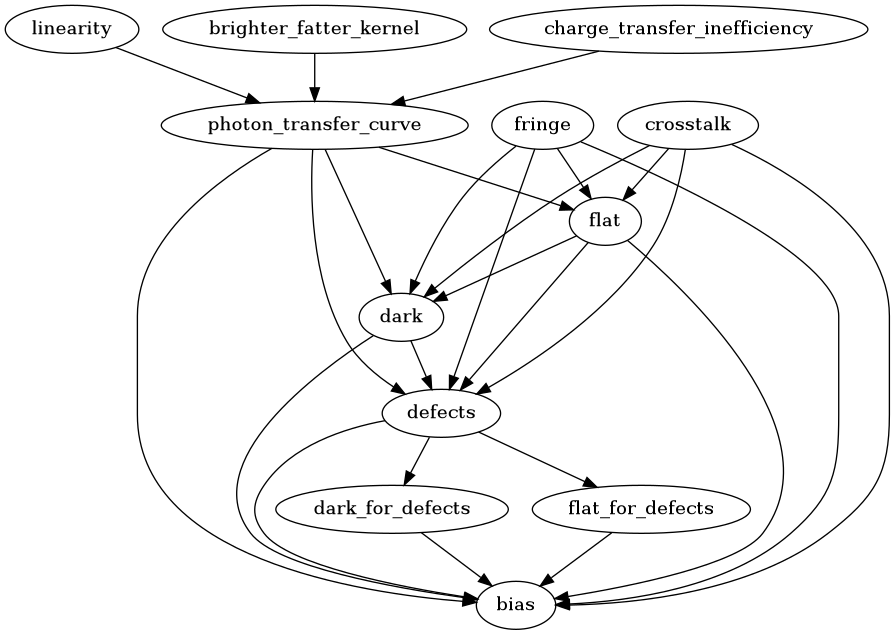
\includegraphics[width=\linewidth]{figures/dependence.png}
  \caption{Dependency charge of calibration products.  The arrow indicates the parent calibration.}
  \label{fig:dependence}
\end{figure}

The \verb|observation_type| and \verb|observation_reason| of the input exposures should match the calibration type to be constructed, with the exception of the fringe and crosstalk calibrations, which are constructed from science exposures.  Most calibrations can be constructed from a single set of daily calibrations, with the number of bias, dark, and flat frames in these sets (generally of order 15-20) sufficient to create a usable combined calibration.  Dense PTC curves will require many more inputs (on the order of 100 pairs of exposures), and we currently expect that we will have dedicated observation sequences for this purpose.

Calibrations constructed for general use should be able to use the version of the \verb|cp_pipe| tasks and pipelines on the main github branch.  It is preferable to keep code development separate from the calibration construction, but it is expected that these will likely be coupled during commissioning.

To ensure all butler repositories have a consistent set of calibrations, we have decided that only one processing location should perform the calibraion construction steps.  The US Data Facility (USDF) is now operational, all calibrations used for the survey will be generated there.  The process for transferring the calibrations to other butler sites is discussed below in Section \ref{sec:calib_export}.

\subsection{Verification}

Once the proposed calibrations have been generated, the calibration should be used for processing using the \verb|cp_verify| tasks and pipelines.  These tasks measure quality metrics from those processed exposures, and identify any test failures.  At a minimum, the exposures used to construct the calibration should be included, as this can identify problematic inputs that degrade the calibration quality.  An example of this is saturated flat exposures, which do not flat-field well, and should not be included in the final flat calibration.  In running the \verb|cp_verify| tasks, the input butler collections specified should have the construction RUN collection placed at the beginning of the list, to ensure that the verification process will find and use the calibration we wish to verify.

Exposures from outside the set used for construction should be added to provide insight into the expected validity range for the calibration.  As long as the metrics on those exposures remain within the limits defined in \citedsp{DMTN-101}, the calibration may continue to be valid for the date range including those additional exposures.  This can be used to establish the valid date ranges to be used when certifying the calibration.

The \verb|cp_verify| pipelines will generate and publish \verb|analysis_tools| ``core'' metrics and plots to cover the \citedsp{DMTN-101} tests.  These metrics and plots will also include useful diagnostic results based on the camera team \verb|eo_pipe| tests.  Further ``extended'' metrics and plots may also need to be generated to supply additional debugging information about the calibrations.

\subsection{Certification}

Once the new combined calibration has been generated and verified, it can be certified for use for a given date range.  Calibrations that have been constructed due to a camera or telescope change, or that are being built to replace another calibration that is no longer within the test specifications, should always have a starting validity date, with the end date left open.  This ensures that future data taken will always have valid calibrations for processing.

If historical calibrations are being constructed, the end date should be known from the daily calibration processing results stored in the visit database (see Section \ref{sec:daily_verify} below).  Future development is needed to allow calibrations to be recertified to update the date ranges.

CZW Todo: example command

\subsection{Approval}

With the calibrations built, verified, and certified, a TAXICAB ``hailing'' ticket should be created, with a verification report (the format of which is to be determined) attached for member consideration.  Any additional processing that is suggested by the TAXICAB should be defined and run prior to the TAXICAB meeting, which will have a planned weekly timeslot.  If no open TAXICAB hailing tickets exist, this meeting will be skipped.

The TAXICAB will consider the verification reports, identify any potential issues with the calibration set, and determine if any verification test failures warrant restarting the construction process to address the issues.  Ideally, all verification metrics will succeed, and a quick check of residual exposures will show no unexpected features.  In the more likely case that some fraction of thesetests fail, the TAXICAB will be tasked with deciding if the failures are fatal and the calibration should be fully rejected, or if the failures are small enough in number or impact that the calibration can be accepted for use despite them.  The TAXICAB will operate on a consensus basis, to ensure that all stakeholders have input on this process.

If the calibrations were built using a ticket/development branch of any software, those code changes must be reviewed and approved through the standard DM process prior to hailing the TAXICAB.  If no new code was added, then the approval of the TAXICAB can be used as the review process to close the initial generation ticket.

CZW Todo: Add a reference to where the TAXICAB is defined.

\subsection{Distribution}

Upon approval of the TAXICAB, the calibrations can be distributed for use.  A separate distribution ticket should be created to handle this work, and linked to both the construction ticket and the TAXICAB ticket.  As the calibrations have already been certified in the origin butler repository, the distribution process for that repository simply needs a CHAINED collection added that contains all of the calibrations generated on the construction ticket.  This new CHAINED collection can then be prepended to the top level calibration CHAINED collection, installing the calibration for use.

The calibrations must then be exported for use in other repositories, with the butler repository at the summit being most important to update. CZW Todo: Update clarify

\begin{verbatim}
butler export-calibs $REPO ./export_directory LATISS/calib/DM-XYZ LATISS/calib/DM-XYZ/voltageChange/bias [...]
\end{verbatim}

This command exports the files into the \verb|export_directory| location, and constructs a YAML description of the calibrations and their collections.  This \verb|export_directory| must then be transferred to the host of the new repository, where it can be imported with the command

\begin{verbatim}
butler import $NEW_REPO  --transfer copy \
       --export-file ./export_directory/export.yaml ./export_directory \
       -s instrument -s detector -s physical_filter
\end{verbatim}

The \verb|--transfer copy| is strongly suggested, as this will copy the files into the repository datastore, removing any dependency on the \verb|export_directory|.  The three \verb|-s| arguments indicate that the \verb|instrument|, \verb|detector|, and \verb|physical_filter| definitions contained the the YAML description should be skipped, as they will already exist in a repository that has been set up for the appropriate camera.

The newly imported collections will not by default be part of the main public calibration collection.  To do so, the new collections must be added to the collection chain.  Using the following command with the `prepend` mode will add the new collections to the start of the collection chain, making them available.

\begin{verbatim}
butler collection-chain $NEW_REPO --mode=prepend LATISS/calib \
       LATISS/calib/DM-XYZ \
       LATISS/calib/DM-ABC
\end{verbatim}

The distribution ticket should be able to be self-reviewed, after confirming that at least one exposure from the validity range of the new calibrations can be processed through \verb|IsrTask|, and that the output processed exposure has the correct calibration information recorded in its header.

\section{Daily Calibrations}

Daily calibrations will be used to monitor the camera and telescope for changes. In general, we expect that the daily calibration  processing will simply verify these newly taken exposures against the existing calibration set as shown in Figure \ref{fig:daily}.  This allows the long-term stability of the calibrations to be monitored.

The verification results from the daily calibration processing will issue (CZW: LOVE?) alarms if any tests fail.  This should notify the TAXICAB members and result in CZW: Someone-to-be-named initiating a new calibration construction process to supply updated calibrations prior to observing (CZW: I don't know the timing of things here).


\begin{figure}
  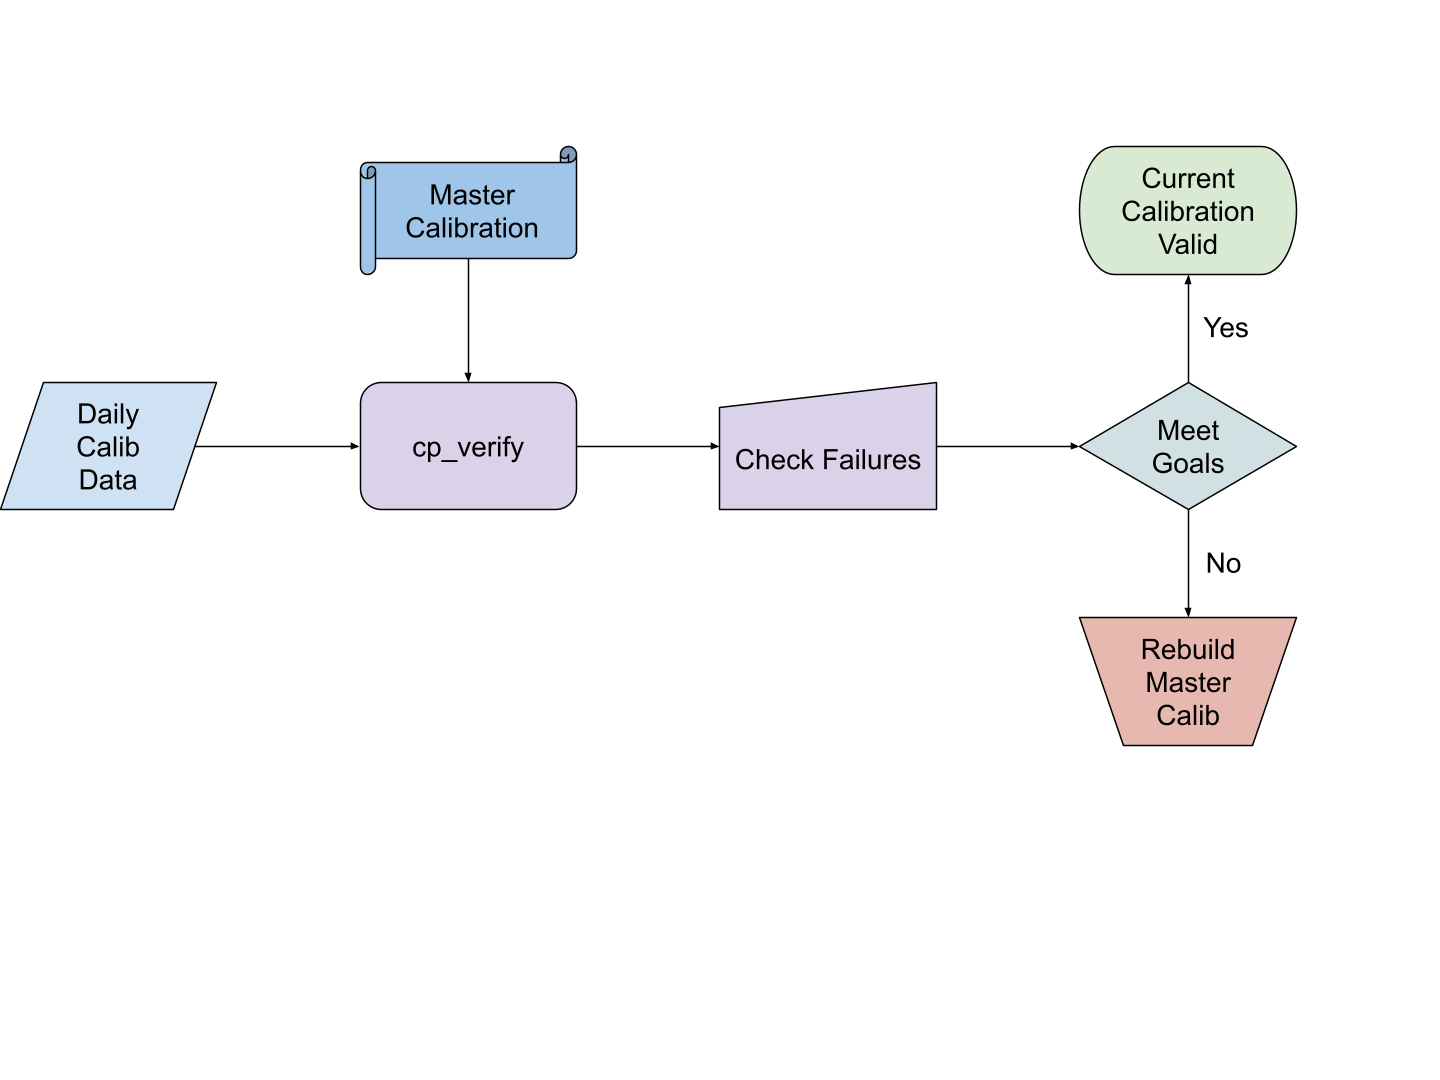
\includegraphics[width=\linewidth]{figures/daily_processing.png}
  \caption{Flowchart of the daily calibration process.}
  \label{fig:daily}
\end{figure}

\section{Curated Calibrations}

Curated calibrations are those calibrations that cannot easily be generated from a series of exposures, or that require special hardware that will not be available at the summit.  Currently, the camera geometry calibration is the only curated calibration in wide use.   These calibrations will be ingested via the \verb|butler write-curated-calibrations| command.  This command by default will attempt to write to the main \verb|$INSTRUMENT/calib| collection.  This is generally not desired, as it is useful for that collection name to point to a CHAINED butler collection, to allow for easier calibration management.  Instead, a ticketed collection name should be used, as the following example illustrates for the LATISS camera.

\begin{verbatim}
butler write-curated-calibrations $REPO lsst.obs.lsst.Latiss \
       --collection LATISS/calib/DM-XYZ --label DM-XYZ
\end{verbatim}

This will ensure that the calibrations can be chained into the main collection as detailed above.


\section{Conclusions}

\appendix
% Include all the relevant bib files.
% https://lsst-texmf.lsst.io/lsstdoc.html#bibliographies
\section{References} \label{sec:bib}
\renewcommand{\refname}{} % Suppress default Bibliography section
\bibliography{local,lsst,lsst-dm,refs_ads,refs,books}

% Make sure lsst-texmf/bin/generateAcronyms.py is in your path
\section{Acronyms} \label{sec:acronyms}
\addtocounter{table}{-1}
\begin{longtable}{p{0.145\textwidth}p{0.8\textwidth}}\hline
\textbf{Acronym} & \textbf{Description}  \\\hline

DM & Data Management \\\hline
DMTN & DM Technical Note \\\hline
LATISS & LSST Atmospheric Transmission Imager and Slitless Spectrograph \\\hline
LOVE & LSST Operations Visualization Environment \\\hline
PTC & Photon Transfer Curve \\\hline
US & United States \\\hline
USDF & United States Data Facility \\\hline
\end{longtable}

% If you want glossary uncomment below -- comment out the two lines above
%\printglossaries





\end{document}
